\documentclass[9pt,twocolumn,twoside]{pnas-new}
% Use the lineno option to display guide line numbers if required.

\templatetype{pnasresearcharticle} % Choose template
% {pnasresearcharticle} = Template for a two-column research article
% {pnasmathematics} %= Template for a one-column mathematics article
% {pnasinvited} %= Template for a PNAS invited submission

% Added by V. Van der Meersch
\usepackage{gensymb}
\newcommand{\textappr}{\raisebox{0.5ex}{\texttildelow}}

\begin{document}
\title{Biological mechanisms are necessary to improve projections of species range shifts}

% Use letters for affiliations, numbers to show equal authorship (if applicable) and to indicate the corresponding author
% Include department, institution, and complete address, with the ZIP/postal code, for each author
\author[a,1]{Victor Van der Meersch}
\author[b]{Edward Armstrong}
\author[a]{Florent Mouillot}
\author[c]{Anne Duputié}
\author[d]{Hendrik Davi}
\author[e]{Frédérik Saltré}
\author[a,1]{Isabelle Chuine}

\affil[a]{CEFE, Univ Montpellier, CNRS, EPHE, IRD, 34000 Montpellier, France}
\affil[b]{Dept. of Geosciences and Geography, University of Helsinki, Helsinki, Finland}
\affil[c]{UMR 8198-EEP-Evo-Eco-Paleo, Université de Lille, CNRS, Lille, France}
\affil[d]{URFM, INRAE, Avignon, France}
\affil[e]{Global Ecology, College of Science and Engineering, Flinders University, Adelaide, Australia}

% Please give the surname of the lead author for the running footer
\leadauthor{Van der Meersch}

% Please add a significance statement to explain the relevance of your work (120-words max)
\significancestatement{While climate change is already reshaping ecosystems around the world, we still have not elucidating which modelling approaches could provide the most reliable projections of species range shifts.  Here, we used multiple models to simulate past tree species distributions across Europe over the last 12,000 years, and evaluated their projections against fossil pollen data. We show that projections of correlative models (the most widely used tools) are less reliable, in more distant and dissimilar climatic conditions, than that of more complex models describing biological processes.
Our findings suggest that biological mechanisms are key in model building to increase the reliability of projections of climate change impacts on biodiversity and ecosystems.}

% Please include corresponding author, author contribution and author declaration information
\authorcontributions{V.V. and I.C. designed research; V.V. and E.W. performed research; V.V., A.D., F.S. and I.C. analyzed data; and V.V., E.W., F.M., A.D., H.D., F.S. and I.C wrote the paper.}
\authordeclaration{The authors declare no competing interests.}
\correspondingauthor{\textsuperscript{1}To whom correspondence should be addressed. E-mail: victor.vandermeersch@cefe.cnrs.fr or isabelle.chuine@cefe.cnrs.fr.}

% At least three keywords are required at submission. Please provide three to five keywords, separated by the pipe symbol.
\keywords{Ecological modelling $|$ model transferability $|$ species range shift}

\begin{abstract}
The recent acceleration of global climate warming has created an urgent need for reliable projections of species distributions, widely used by natural resource managers. Such projections, however, are produced using various modeling approaches with little information on their relative performances under expected novel climatic conditions. Here, we hindcast the range shifts of five forest tree species across Europe over the last 12,000 years to compare the performance of three different types of species distribution models and determine the source of their robustness. We show that the performance of correlative models (CSDMs) decreases twice as fast as that of process-based models (PBMs) when climatic dissimilarity rises, and that PBM projections are likely to be more reliable than those made with CSDMs,  at least until 2060 under scenario SSP245. These results reveal the major importance of describing biological mechanisms explicitly to ensure model robustness, and highlight a new avenue to improve model projections in the future.
\end{abstract}

\dates{This manuscript was compiled on \today}
\doi{\url{www.pnas.org/cgi/doi/10.1073/pnas.XXXXXXXXXX}}


\maketitle
\thispagestyle{firststyle}
\ifthenelse{\boolean{shortarticle}}{\ifthenelse{\boolean{singlecolumn}}{\abscontentformatted}{\abscontent}}{}

\firstpage[7]{5}
% Use \firstpage to indicate which paragraph and line will start the second page and subsequent formatting. In this example, there are a total of 11 paragraphs on the first page, counting the first level heading as a paragraph. The value {12} represents the number of the paragraph starting the second page. If a paragraph runs over onto the second page, include a bracket with the paragraph line number starting the second page, followed by the paragraph number in curly brackets, e.g. "\firstpage[4]{11}".


% If your first paragraph (i.e. with the \dropcap) contains a list environment (quote, quotation, theorem, definition, enumerate, itemize...), the line after the list may have some extra indentation. If this is the case, add \parshape=0 to the end of the list environment.
\dropcap{M}odelling is essential for understanding and predicting  the impacts of  climate change on ecosystems and biogeochemical cycles. Credible model projections are critical for natural resource managers, decision makers and stakeholders to make informed decisions. To meet the demand for reliable projections of ecosystems and biodiversity dynamics, comprehensive assessments  of ecological model performances must be a priority \cite{Dawson2011, Mouquet2015, Pacifici2015}. 

One approach to evaluate model reliability is to compare their predictions to observations from previous time periods, i.e. hindcasting. Hindcasting can inform whether models capture, implicitly or explicitly, the essential processes required to provide reliable projections in conditions significantly different from the present. By looking far into the past, paleo-archives have proven to offer a unique opportunity to both understand long-term climate and biodiversity dynamics \cite{Bartlein2011, Fordham2020} and test model robustness and transferability (i.e. model capacity to maintain its performance in changing conditions \cite{UribeRivera2023}) \cite{Braconnot2012, Maguire2015}.  

Yet, models prediction of past species distribution and biospheric components have rarely been consistent with paleoclimate reconstructions and fossil records \cite{Veloz2012, Pearman2008, Roberts2012, Foley2013, Maguire2016} . Interpreting model projections in climatic conditions that differ significantly from the present, such as future no-analogue climatic conditions \cite{Williams2007}, remains challenging. Therefore, the guarantee that ecological model forecasts for the 21\textsuperscript{st} century will be reliable is limited \cite{Fitzpatrick2018}. 

While exact matches to expected 21\textsuperscript{st}-century climatic conditions do not exist in historical records \cite{Burke2018}, the dissimilarity between 20\textsuperscript{th} and 21\textsuperscript{st} century median climatic conditions (Material and Methods) falls within the range of dissimilarity encountered since the beginning of the Holocene (12 kyr BP, with kyr = 1000 years and BP = Before Present (1950); \hyperref[fig:climaticdissimilarity]{Fig. 1}). This period takes place after the Last Glacial Maximum (26.5-19 kyr BP \cite{Clark2009}) and began with an abrupt climate warming followed by a long, almost uninterrupted, period of climatic stability until recent anthropogenic warming (Fig. S1). The fossil pollen data accumulated over these last millennia provides us with an unique extended timeframe to test the reliability of ecological models, in particular those designed to predict changes in species distribution.

Species distribution models (SDM) are powerful tools to predict species geographical distribution as a function of environmental data (e.g., mean annual temperature and annual total precipitation). Most studies have focused on correlative models (CSDMs, also called environmental niche models), which infer statistical relationships between observations of species occurrences and environmental predictors \cite{Dormann2012}. Their high flexibility and low computational complexity make them the most widely used tool for deciding on species conservation plans and policy regimes (e.g. \cite{Hanewinkel2013}). However, under novel climatic conditions, new unobserved portions of a species’ climatic niche may appear, which are not captured by these correlative (or phenomenological) approaches. For example, when tested under distant past climates, the predictive performance of CSDMs  significantly decreased \cite{Maguire2016}, questioning their ability to provide reliable projections in the future \cite{Fitzpatrick2018}. 

\begin{figure*}%[tbhp]
\centering
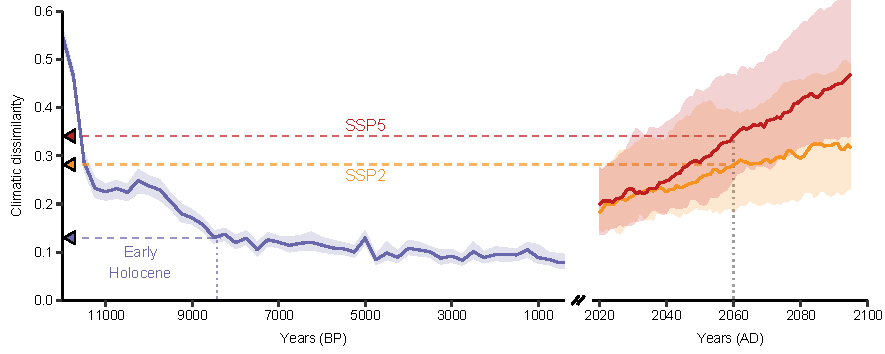
\includegraphics[width=17cm]{climatic_dissimilarity-1.pdf}
\caption{Evolution of climatic dissimilarity during the Holocene (12k-500 yr BP) and the 21st century (2005-2100), relative to 1901-2000. Climatic dissimilarity is computed as 1-Sørensen similarity between bootstrapped climatic hypervolumes. Lines represent median dissimilarity, shaded areas represent 90\% confidence intervals. Blue corresponds to paleoclimate based on HadCM3B model. Yellow and red correspond to future climatic conditions according to SSP245 and SSP585 scenarios respectively, predicted by 34 global climate models of NEX-GDDP-CMIP6. The blue triangle on y-axis indicates the level of climatic dissimilarity 8500 years ago, at the limit between the Early and Late-Middle Holocene. Yellow and red triangles indicate the expected level of climatic dissimilarity in 2060 for SSP245 and SSP585 scenarios. Note that the x-axis scale is different between past and future panels.}
\label{fig:climaticdissimilarity}
\end{figure*}

Alternative approaches to CSDMs are process-based models (PBMs, or process-explicit models) that rely on explicit formulations of the mechanisms driving the distribution of a given species (e.g., physiological, ecological and/or demographic processes). They come from decades of experiments and observations, including extreme conditions in laboratory \cite{Seehausen2017}, and climate manipulations such as CO\textsubscript{2} enrichment \cite{Jiang2020} or rainfall exclusion \cite{Gavinet2019}. The reliability of PBMs depends on our level of understanding of how environmental conditions affect ecophysiological processes, and the availability of large amount of observations to calibrate their many parameters \cite{Evans2016}. Because these models do not rely on statistical relationships between present-day species occurrences (presence/absence) and environmental variables, but rather describe explicit causal relationships between biological processes and environmental variables, they are believed to provide more reliable predictions of species distribution changes under novel climatic conditions  \cite{Evans2012, Singer2016}. However, another possible reasons why PBM projections might be more reliable than CSDM projections under novel climatic conditions could also come from their calibration methods. Unlike CDSMs that are calibrated using species presence/absence data, PBM parameters are either measured directly (e.g. specific leaf area, leaf frost hardiness), or inferred statistically when direct measurement is not an option, using data on specific functional traits measured in the field or in laboratory (e.g. parameters of bud dormancy break date models). 

Despite the growing interest for PBMs in predictive ecology \cite{Connolly2017, Urban2016, Pilowsky2022}, the widespread assumption that they provide more reliable projections of future species range shifts has yet to be verified. Furthermore,  the reasons behind this assumption have not been clearly articulated. Qualitative models comparison under future climatic conditions have shown that PBMs often make more conservative projections in future climates than CSDMs which predict larger changes \cite{Morin2009, Cheaib2012, Gritti2013} but they have not provided any confidence level in these results. Very few studies have actually gone beyond qualitative comparisons between CSDMs and PBMs and compared thoroughly their performance, for example using virtual species \cite{Zurell2016}, exotic species in native and newly colonized areas \cite{Higgins2020}, or in the recent past \cite{Fordham2018}. 
While PBMs have shown their usefulness for paleoecological studies \cite{Saltre2013, Ruosch2016, Schwoerer2014}, the extent to which they can provide more reliable predictions than CSDMs under different climatic conditions from the historical period remains unknown \cite{UribeRivera2023, Briscoe2019}. 

Here, we address this critical gap by using multiple CSDMs and PBMs to simulate paleodistributions of five emblematic tree species of Europe at a high temporal resolution since 12 kyr BP. We used daily paleoclimatic data at 0.25° spatial resolution, generated from HadCM3B-M2.1 coupled general circulation model simulations, which includes both inter-annual variability, and millennial scale variability for rapid Dansgaard–Oeschger events before 11 kyr BP \cite{Armstrong2019}. Species migration ability was also incorporated into the simulations to represent more comprehensively changes in species' realized distribution and not merely changes in their climatic niches to allow for a more  accurate comparison with the paleorecords.

We first assessed which modelling approach best predicts past species distributions, and second whether model performance was related to their hypotheses (relationships describing explicit biological mechanisms or not) or to their calibration methods (calibrated on species occurrence data or not). To do so, we compared three types of models: CSDMs, PBMs (hereafter called expert PBMs) and fitted PBMs calibrated in the same way as CSDMs (inverse calibration using species occurrence data and a novel type of algorithm; Material and Methods and \cite{VanderMeersch2023}). The comparison between CSDMs/fitted PBMs and expert PBMs allowed us to determine whether the differences in model performance arise from their calibration methods, whereas the comparison between CSDMs and expert/fitted PBMs allowed us to determine whether the differences in model performance arise from the model hypotheses. We assessed the performance of the models for the maximum level of climate dissimilarity possible, i.e. over the last 12,000 years, which corresponds to the climate dissimilarity expected by the end of the century according to SSP245, and by the middle of the century according to SSP585 (\hyperref[fig:climaticdissimilarity]{Fig. 1}).

\begin{figure}
\centering
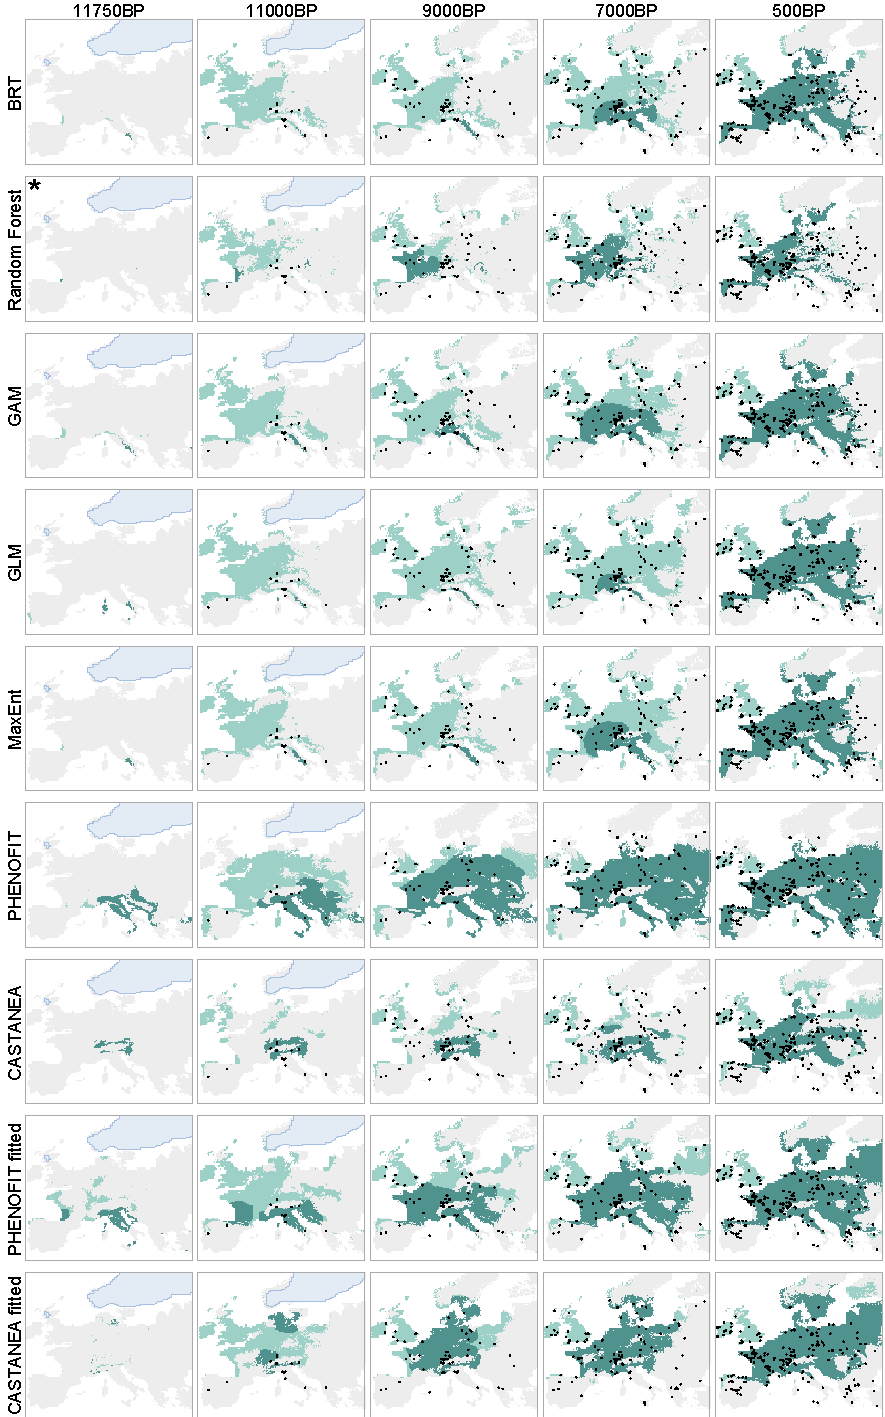
\includegraphics[width=0.95\linewidth]{quercus_deciduous_simulations-1.pdf}
\caption{Example of paleosimulations obtained with the nine models used in this study for deciduous oaks. The five first rows correspond to the five correlative models (boosted regression tree, down-sampled random forest, generalized additive model, generalized linear model with lasso regularization, MaxEnt). The four last rows correspond to two different versions (expert calibration and inverse calibration using occurrence data) of two process-based models (PHENOFIT and CASTANEA). Light green area is the modelled suitable area, dark green area is the colonized area (after migration). Light blue represents the ice sheet extent. Black dots are deciduous oak fossil pollen occurrences. The model for which migration started at 11.75 kyr BP rather than 12 kyr BP is marked with an asterisk. "BP" stands for "before present" (1950).}
\label{fig:quercusdeciduoussimulations}
\end{figure}

\section*{Results}
% add something about future somewhere? 
As observed in previous long-term historical assessments, all models showed a decrease of their performance when moving further into the past, i.e. into more different climatic conditions than historical conditions (\hyperref[fig:pastperformance]{Fig. 3a}). However PBMs showed smaller decrease in their predictive performance (slope of Beta regression, fitted PBMs: $-6.07$, 95\% CI $[-8.62, -3.55]$, expert PBMs: $-4.44$, 95\% CI $[-7.07, -1.77]$) than CSDMs ($-11.0$, 95\% CI $[-13.2, -8.91]$). PBMs also showed higher transferability in the most distant climatic conditions of the early Holocene than CSDMs (\hyperref[fig:pastperformance]{Fig. 3d}). PBMs, either expert or fitted, are thus less affected by the increase in climate dissimilarity than CSDMs. In the near past (Late-Middle Holocene, $<$ 8.2 kyr BP), CSDMs were not significantly better at predicting tree distribution than any PBMs (pairwise Conover-Iman tests: \emph{vs.} expert PBMs \emph{t}-statistic $=1.68$/\emph{P} $=0.128$, \emph{vs.} fitted PBMs \emph{t}-statistic $=-1.55$/\emph{P} $=0.112$; \hyperref[fig:pastperformance]{Fig. 3b}), despite their closer fit to current species distributions (Fig. S8). In the distant past (Early Holocene $>$ 8.2 kyr BP), CSDMs performed worse than both expert and fitted PBMs (pairwise Conover-Iman tests: respectively \emph{t}-statistic $=-4.80$/\emph{P} $<0.0001$ and \emph{t}-statistic $=-5.07$/\emph{P} $<0.0001$; \hyperref[fig:pastperformance]{Fig. 3b}). The maximum climatic dissimilarity during this period corresponds to the climatic dissimilarity expected as soon as 2060 according to the scenario SSP245 (\hyperref[fig:pastperformance]{Fig. 3a}).

These differences between PBMs and CSDMs are closely related to their ability to predict species recolonisation dynamics in the Early Holocene (\textappr11.5-8.5 kyr BP). Both types of PBMs, fitted and expert, predicted more accurately refugia locations at -12 kyr BP, which were the starting points for the migration (\hyperref[fig:quercusdeciduoussimulations]{Fig. 2}; Material and Methods). This period corresponds to a global deglaciation which lasted for a few centuries and occurred after the cooling of the Younger Dryas interval  (\textappr13-11.5 kyr BP; Fig. S1). This rapid warming episode explains the strong decrease of climate dissimilarity relative to present between 12 kyr BP and 11.5 kyr BP (\hyperref[fig:climaticdissimilarity]{Fig. 1}). If we had not considered the 12-11.5 kyr BP period of high climatic dissimilarity (i.e. without simulating migration from refugia), we would have missed the opportunity to take into account model projections within the same dissimilarity level to what we expect between 2050 and 2100 (\hyperref[fig:climaticdissimilarity]{Fig. 1}). When models are compared after 11kyr BP, i.e. when climate dissimilarity is more similar to present, CSDMs and PBMs' abilities to predict fossil pollen occurrence are similar (Fig. S10cd), with an average Sørensen index decrease of $-0.205\pm0.0224$ (paired Wilcoxon-test: \emph{P} $<0.0001$) between Late-Middle Holocene and Early Holocene.

\begin{figure*}[tbhp]
\centering
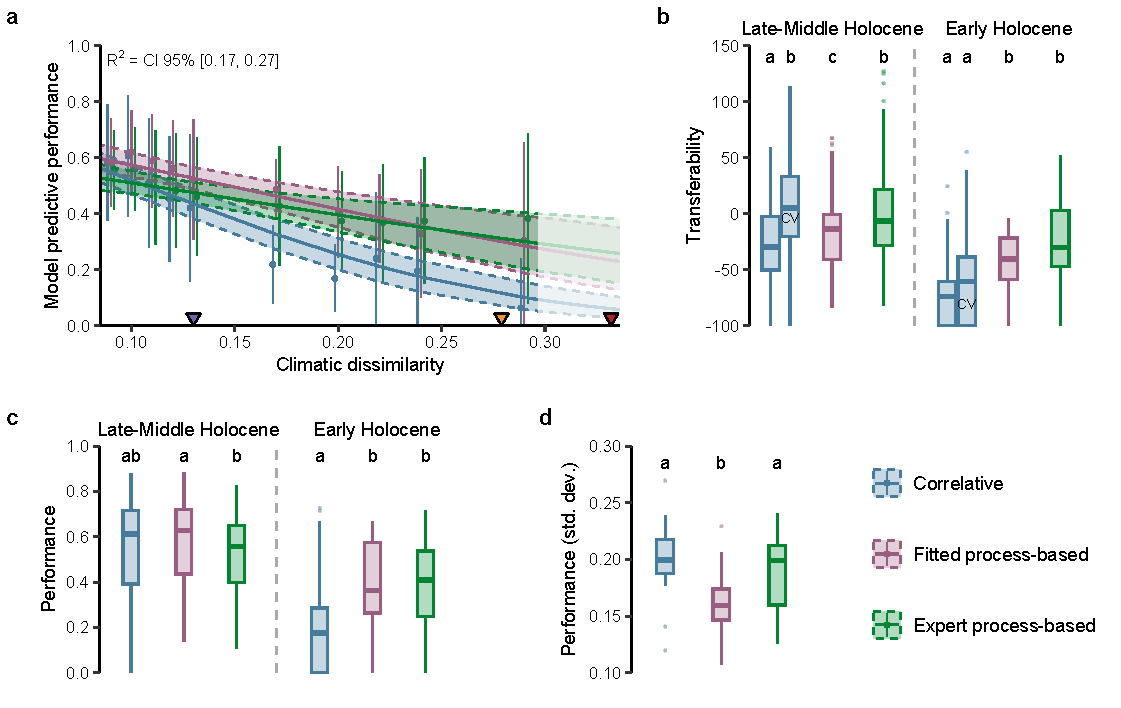
\includegraphics[width=17cm]{past_performance.pdf}
\caption{Performance of correlative models, fitted process-based models (inverse calibration using occurrence data) and expert process-based models (classical calibration) against Holocene paleoecogical evidence (fossil pollen) for 4 tree genera (\emph{Abies}, \emph{Fagus}, \emph{Quercus} deciduous and \emph{Quercus} evergreen). \textbf{(a)} Bayesian beta regression of model predictive performance (Sørensen index) against climatic dissimilarity relative to 1901-2000 (1-Sørensen similarity between climatic hypervolumes). Shaded areas represent 2.5\% and 97.5\% quantiles of the posterior predictive distribution. Points represent the average model performance (and lines the standard deviation) grouped by similar level of climatic dissimilarity. Blue triangle on x-axis indicates the limit between Early Holocene ($>$ 8.2 kyr BP) and Late-Middle Holocene ($<$ 8.2 kyr BP). Yellow and red triangles indicate the expected level of climatic dissimilarity in 2060 for SSP245 and SSP585 scenarios. Legend on the right: top row represents drivers of modelled distributions (correlations/mechanisms), bottom row represents calibration method (species distributions/measurements). Panels \textbf{(b)} and \textbf{(c)} show the difference in performance (Sørensen index) and variability in performance (standard deviation of Sørensen index) across models. Panel \textbf{(d)} shows the transferability of the models (relative change in model performance between distant past periods and historical period). A negative transferability means that model performance is lower in the distant past periods than in the historical period. CSDM predictive errors in the historical period was assessed by two different methods: (i) against the same data used for calibration (leading to an overestimation of historical model performance -- but more comparable to fitted PBM estimates), (ii) using an environmental block cross-validation, noted as "CV" (leading to a better estimation of true model errors in the historical period, and thus a higher transferability -- but less comparable to fitted PBMs for which cross-validation would have been too computationally expensive). The grouping letters represent the multiple comparisons with pairwise Conover-Iman tests.}
\label{fig:pastperformance}
\end{figure*}

Our results also revealed that inverse calibration improved process-based projections in recent past
without altering significantly PBM long-term transferability (\hyperref[fig:pastperformance]{Fig. 3}). In Middle-Late Holocene, when climate conditions were not drastically different from present, performances of fitted PBMs was higher than those of expert PBMs (\emph{t}-statistic $=2.70$/\emph{P} $=0.020$). In most distant climatic conditions of Early Holocene, their performances were similar (\emph{t}-statistic $=0.220$/\emph{P} $=0.757$; \hyperref[fig:pastperformance]{Fig. 3b}). 

Models performances were not stable across species, and exhibited both similarities and differences across time (Fig. S9). More specifically, models exhibited the same overall performance decrease against \emph{Fagus} pollen records, whereas CSDM performance decline was substantially faster than expert and fitted PBMs for deciduous \emph{Quercus}. All models show low predictive power regarding evergreen \emph{Quercus} distribution even in the Late Holocene compared to other species, especially CSDMs which failed to predict its presence along the Atlantic coast (S6). Fitted PBMs, however, showed the lowest variability of performance across species (\hyperref[fig:pastperformance]{Fig. 3c}).


\section*{Discussion}

Our results suggest that the transferability and robustness of models are more strongly influenced by the processes explicitly represented within the models than by their method of calibration. PBMs consistently show a better performance throughout the 12 kyr simulation period, even when calibrated using the same method as CSDMs. Therefore, beyond enabling a more detailed mechanistic understanding of the effects of environmental conditions on species survival, growth, and reproduction, biological processes represented in PBMs are critical to ensure higher model robustness under more novel climatic conditions. This important new finding advocates for a wider use of PBMs to predict biodiversity and ecosystems distributions in the future and opens a new avenue to reach this goal by using inverse modelling approaches to calibrate them.

Our results also suggest that predictions of PBMs, either fitted or expert, should be more reliable at least up to 2060 according to the scenario SSP245 (\hyperref[fig:pastperformance]{Fig. 3a}) and 2050 according to SSP585. The rate of anthropogenic climate change and the increased probability of occurrence of novel climates (\cite{Williams2007}; \hyperref[fig:climaticdissimilarity]{Fig. 1}) are challenging the reliability of both CSDMs and PBMs especially when they are intended to be used in more complex models such as biosphere-atmosphere models and by natural resource managers and policy makers to guide management plans and policies. Acknowledging these uncertainties is as important as making the forecasts themselves \cite{Beale2012} and contributes to the public trust in scientists \cite{Berkhout2010}.

Simulating migration allowed us to take into account the differences between the models under the most challenging conditions, i.e., when the climate dissimilarity was at its greatest, closely approximating what is projected for  the end of the 21st century. Since the migration model is identical across all simulations, differences of performance between models across the Holocene very much depended on their ability to predict the potential refugia of the species during the Early Holocene. For example, some models were not able to predict evergreen \emph{Quercus} refugia in Southern Spain, thus missed an important migration route and failed predicting their presence in vast areas in the Late Holocene (Fig. S6). As PBMs, either fitted or expert, describe the response of ecophysiological processes to a wide range of environmental conditions, they can provide a better estimate of the environmental conditions in which species could have survived 12000 years ago, under climates much more dissimilar to present conditions. A potential limitation of our approach though is that we cannot account for very rare and really long-distance dispersion events, as well as the influence of humans. For example all models failed to predict deciduous \emph{Quercus} in the British Isles before the Early Holocene sea level rise and the opening of the Strait of Dover (\hyperref[fig:quercusdeciduoussimulations]{Fig. 2} and \cite{Smith2011}), even though the land-sea mask changed throughout the simulations. It remains unclear whether this failure is due to the models' misrepresentation of very long-distance dispersion events of seeds (e.g. by humans or jays, across major dispersal barrier), or a consistent misprediction by all models of more northern refugia.

The recent efforts to gather fossil pollen data and make them openly available \cite{Williams2018} allow us to objectively assess model performance under climate conditions vastly different from those used for their calibration. From 11.5 kyr BP onwards, climate dissimilarity varies between 0.29 and 0.08, a level equivalent to what we might experience in the second quarter of the 21st century (\hyperref[fig:climaticdissimilarity]{Fig. 1}). Model consistency with past observations does not demonstrate that the model will be valid in the future \cite{Oreskes1994}, but we make here a critical step towards enhancing our understanding of model transferability. As more and more pollen data becomes available, we could cover a wider range of conditions, prior 11.5 kyr BP.
% Incorporating migration has nevertheless enabled us to observe that the accuracy of the starting point of the simulations at 12 kyr BP,  played a major role in assessing the performance of the models throughout the Holocene. 
Our simulations have nevertheless started at 12 kyr BP, when climatic dissimilarity was at its highest, and transitioned to a climate more analogous to historical state. The uncertainties on the initial conditions had thus a significant influence on the simulation outcomes. In the future, on the contrary, initial uncertainties will be much lower as models will start from the known distributions of species. However, uncertainties will increase as simulations proceed towards increasingly dissimilar climatic conditions, especially since these conditions  will extent beyond the range experienced in the past (Fig. S3).

While quantifying the uncertainty in model projections remains challenging, our results pave the way for drastic improvement in model evaluation. The discrepancies between model performances we observed highlights the importance of considering various modelling methods to capture the full range of uncertainties associated with future projections. It implies that we should not rely solely on the model's own prediction dispersion to estimate projection uncertainties, nor on very similar modelling approaches, especially when climate dissimilarity sharply increases. Moreover, models will have to consider that tree colonization dynamics will likely be very different in the future because it will not only occur from a few refugia but from wider continuous ranges, and direct anthropogenic factors, such as sylvicultural practices and assisted species migration, will also shape the composition of forests \cite{Aitken2016}.

Fitted PBMs bring together the strengths from both CSDMs and expert PBMs approaches by describing causal relationships between environmental conditions and species performance (i.e. from process-based approaches) and precise estimates of parameter values (from correlative approaches). The differences between expert and fitted PBMs in the Middle-Late Holocene pinpoint some issues in expert parameterization that requires to combine various methods to cope with both the scarcity of data for each ecophysiological process modelled and sometimes non-measurable parameters (e.g. \cite{DeCaceres2023}).  Some parameters in these relations can be measured directly, and exhibit little variability across a species range (e.g. water potential leading to 50\% of vessels embolism). However, the measurement of parameters in controlled conditions does not necessarily guarantee their external validity \emph{in natura} \cite{Asse2020} where numerous factors, not represented in laboratory conditions, can also affect the process modelled (but see \cite{Satake2013}). Other parameters are either highly variable because of local adaptation over long period,  difficult-to-measure or so far unmeasurable (e.g. bud dormancy). Therefore, expert PBMs can suffer from uncertainties entailed in the measurements of some of their parameters, and from spurious data specific to few locations which do not represent sufficiently well all the conditions the species can experience all over its range. For these reasons, inverse calibration presents a valuable opportunity to estimate the values of PBM parameters especially difficult to estimate otherwise \cite{Evans2016, Hartig2014}. However, inverse calibration does not warranty the correct estimation of parameter values and needs to be used critically and with caution \cite{VanderMeersch2023}. 

Our unique multi-model comparison across the Holocene demonstrates that our understanding of biological mechanisms embedded into process-based models represent a real advantage over the empirical relationships used in CSDMs to increase projections reliability for the coming decades. However, data availability limits our ability to parameterize these models, and could explain the difficulty to use them more widely for global impact studies. Fitted PBMs may overcome this problem by using more data at a larger geographical scale, while keeping the predictive strength of causal relationships. Given ongoing improvements in computational methods and the availability of new global-scale measurements (e.g. forest structure and growth with remote sensing and LiDAR data), there is clear opportunity for an extensive calibration and application of process-based models to provide more reliable projections in the coming decades.

% \subsection*{Author Affiliations}

% Use lower case letters to match authors with institutions, as shown in the example. PNAS strongly encourages authors to supply an \href{https://orcid.org/}{ORCID identifier} for each author. Individual authors must link their ORCID account to their PNAS account at \href{http://www.pnascentral.org/}{www.pnascentral.org}. For proper authentication, authors must provide their ORCID at submission and are not permitted to add ORCIDs on proofs.

% \subsection*{Submitting Manuscripts}

% All authors must submit their articles at \href{http://www.pnascentral.org/cgi-bin/main.plex}{PNAScentral}. If you are using Overleaf to write your article, you can use the ``Submit to PNAS'' option in the top bar of the editor window.

% \subsection*{Format}

% Many authors find it useful to organize their manuscripts with the following order of sections: title, author line and affiliations, keywords, abstract, significance statement, introduction, results, discussion, materials and methods, acknowledgments, and references. Other orders and headings are permitted.

% \subsection*{Manuscript Length}

% A standard 6-page article is approximately 4,000 words, 50 references, and 4 medium-size graphical elements (i.e., figures and tables). The preferred length of articles remains at 6 pages, but PNAS will allow articles up to a maximum of 12 pages.

% \subsection*{Digital Figures}

% EPS, high-resolution PDF, and PowerPoint are preferred formats for figures that will be used in the main manuscript. Authors may submit PRC or U3D files for 3D images; these must be accompanied by 2D representations in TIFF, EPS, or high-resolution PDF format. Color images must be in RGB (red, green, blue) mode. Include the font files for any text.

% Images must be provided at final size, preferably 1 column width (8.7cm). Figures wider than 1 column should be sized to 11.4cm or 17.8cm wide. Numbers, letters, and symbols should be no smaller than 6 points (2mm) and no larger than 12 points (6mm) after reduction and must be consistent.

% Figures and tables should be labelled and referenced in the standard way using the \verb|\label{}| and \verb|\ref{}| commands.

% Figure \ref{fig:frog} shows an example of how to insert a column-wide figure. To insert a figure wider than one column, please use the \verb|\begin{figure*}...\end{figure*}| environment. Figures wider than one column should be sized to 11.4 cm or 17.8 cm wide. Use \verb|\begin{SCfigure*}...\end{SCfigure*}| for a wide figure with side legends.

%\begin{SCfigure*}[\sidecaptionrelwidth][t!]
%\centering
%\includegraphics[width=11.4cm,height=11.4cm]{frog.pdf}
%\caption{This legend would be placed at the side of the figure, rather than below it.}\label{fig:side}
%\end{SCfigure*}

% \subsection*{Supporting Information Appendix (SI)}

% Authors should submit SI as a single separate SI Appendix PDF file, combining all text, figures, tables, movie legends, and SI references. SI will be published as provided by the authors; it will not be edited or composed. Additional details can be found in the \href{https://www.pnas.org/authors/submitting-your-manuscript#manuscript-formatting-guidelines}{PNAS Author Center}. The PNAS Overleaf SI template can be found \href{https://www.overleaf.com/latex/templates/pnas-template-for-supplementary-information/wqfsfqwyjtsd}{here}. Refer to the SI Appendix in the manuscript at an appropriate point in the text. Number supporting figures and tables starting with S1, S2, etc.

\matmethods{
\subsection*{Correlative and process-based models}\label{models}

We used PHENOFIT and CASTANEA, two process-based models which differ by their underlying hypothesis and complexity. 
PHENOFIT simulates the fitness of an average adult tree \cite{Chuine2001}. It estimates fitness components (survival and reproductive success) by simulating the precise phenology (dates of leaf unfolding, flowering, fruit maturation, leaf senescence) and damages caused by abiotic stress (frost, drought) which effects depend on their occurrence relatively to the development stages of the different organs. It has been validated for several North American and European species \cite{Morin2007, Saltre2013, Duputie2015, Gauzere2020}. The model has \textappr30 parameters. 
CASTANEA simulates carbon and water cycles of an average adult tree by simulating many processes such as photosynthesis, stomatal opening, maintenance and growth respiration, transpiration and carbon allocation  \cite{Dufrene2005}. It has been used to predict carbon and water budgets of several European species \cite{Davi2006, Delpierre2012, Davi2017}. 
The model has \textappr80 parameters. 
Both models require daily meteorological variables and soil characteristics. 
%emw13Jan -- The below needs to be clearer for readers in the main text I think. 
Two versions of both models were employed: one was calibrated with expert knowledge and statistical inference using observations and measurements of the processes modelled (version called \emph{expert}), and a second one was entirely calibrated using species distribution data (version called \emph{fitted}, \cite{VanderMeersch2023}) like correlative models. For the latter, we used the optimization algorithm CMA-ES \cite{Hansen2001} as described in \cite{VanderMeersch2023}, and retained the best calibrations in terms of AUC.
  
We selected correlative models based on the thorough model comparison made by Valavi et al. \cite{Valavi2022}. Among the most performant models, we selected five well-established models: GLM with lasso regularization, GAM, BRT, MaxEnt and down-sampled Random Forest. Some of these models are known to struggle when applied to extrapolation domains, but are nevertheless widely used by ecologists to provide projections of species distribution change in future climatic conditions.
We chose four uncorrelated climate predictors related to ecological processes to calibrate these models: minimum temperature of the coldest month (representing frost tolerance), total precipitation (representing available water), GDD5 (growing degree days  \textgreater5°C) between April and September (representing available thermal energy for vegetation growth and fruit maturation), water balance between June and July (precipitation$-$evapotranspiration, representing summer drought tolerance). We also included two soil covariates (pH and Water Holding Capacity).
  
While by construction correlative models directly output species habitat suitability, we used fitness predicted by the model PHENOFIT and net primary production predicted by the model CASTANEA as a proxy of species habitat suitability as they have already been used to predict species presence in previous studies \cite{Morin2009, Cheaib2012, Saltre2013}. 
CSDMs and inverse-calibrated PBMs were calibrated for five species (\textit{Fagus sylvatica} L., \textit{Abies alba} Mill., \textit{Quercus robur} L., \textit{Quercus petraea}  (Matt.) Liebl. and \textit{Quercus ilex} L.) using historical climate (1970-2000) extracted from ERA5-Land hourly dataset \cite{MunozSabater2021}, soil data from EU-SoilHydroGrids \cite{Toth2017} and SoilGrids \cite{Hengl2017} databases and species presence data from the dataset assembled in \cite{VanderMeersch2023}, mostly based on EU-Forest inventory data \cite{Mauri2017}. To calibrate the CSDMs, we additionally sampled 50,000 background points, which should properly represent the variation in the environmental conditions across the study area \cite{Valavi2022}. For each CSDM and each species, we run a fivefold environmental cross-validation to estimate model performance in novel extrapolation conditions (Fig. S8 and \cite{Roberts2017}). We then used all the available training data to calibrate the models for the hindcasting in order to favour final prediction quality \cite{Roberts2017}. We could not run the same cross-validation method for fitted process-based models because it would have been too computationally expensive. 

Model simulations over the Holocene were run for 30-year periods every 250 years, for the five above mentioned species. Model outputs were averaged over each 30-year period. Note that soil conditions (needed both for correlative and process-based models) were held constant throughout the simulations, and were bilinearly interpolated from closest coastal cells where data was missing (because of different land-sea masks between present and past). Note also that for CASTANEA model, species-specific thresholds of net primary production determining the presence or absence of the species were computed with the CO$_2$ level at the beginning of the Holocene (\textappr240ppm).

\subsection*{Late Quaternary climate and vegetation}\label{paleodata}
%emw13Jan -- are there multiple initial conditions (members)? Not critical, I am just wondering. 
We used the monthly paleoclimate simulation dataset \cite{Armstrong2019} generated with the HadCM3B-M2.1 coupled general circulation model, starting from 18 kyr BP at 0.5\degree~spatial resolution for Europe (Fig. S1). We chose this dataset for several reasons. First, it includes both inter-annual variability, and millennial scale variability for rapid Dansgaard–Oeschger events before 11 kyr BP. Second, it shows generally a good agreement with ice-core datasets \cite{Armstrong2019}. Third, it provides all the necessary input variables necessary to run all the models selected.  For this work, several variables were specifically produced: mean temperature, average minimum and maximum daily temperatures, precipitation, number of rainy days, cloudiness, and wind speed. We further downscaled temperature and precipitation monthly data to 0.25\degree~resolution, by applying an elevation correction of coarse-scale variables towards the ICE-6G-C elevation level at high resolution \cite{Peltier2015}.  
We then generated daily data for temperatures, precipitation, cloud cover and wind speed from  the monthly data with the weather generator GWGEN \cite{Sommer2017}, for 30-year periods every 250 years. We also simulated daily extra-terrestrial solar radiation with the same orbital forcing conditions used in HadCM3B-M2.1 \cite{Armstrong2019} and then computed daily global radiation taking into account previously generated daily cloud-cover data as implemented in LPJ-LMfire global model \cite{Pfeiffer2013}. Finally, we computed daily potential evapotranspiration following the standard FAO Penman-Monteith method \cite{Allen1998}.  

Fossil pollen records were extracted from the LegacyPollen dataset \cite{Herzschuh2022}. This dataset is mainly based on the Neotoma database \cite{Williams2018}, and provides samples with standardized chronologies and age uncertainties. We removed sites that had marine depositional environments \cite{Maguire2016}, and only kept samples with more than 200 pollen grain counts and age uncertainty of less than 500 years.
Pollen relative abundances were aggregated to consecutive 500-year intervals. If multiple samples from the same site belonged to the same period, we averaged their pollen abundances, weighting by their age uncertainty and temporal distance from the center of the period. Relative pollen abundances were converted to presence/absence using thresholds based on biome reconstructions \cite{Williams1998}: 1\% for \emph{Fagus} and \emph{Abies}, and 2.5\% for \emph{Quercus}. If several sites fell within the same grid cell (0.25\degree), we considered the species as present if there was at least one site where the species could be considered as present. \textit{Fagus} pollen data were used to assess the presence of \textit{Fagus sylvativa} L., sole species of the genus present in Europe. \textit{Abies} pollen data were used to assess the presence of \textit{Abies alba} Mill., most abundant and widespread fir species present in Europe. When possible, deciduous and evergreen \textit{Quercus} pollen were distinguished based on Neotoma data. Some \textit{Quercus} pollen remain undetermined beyond the generic level, either because discrimination between evergreen and deciduous oak pollen was impossible or because authors were not specific. They were assigned to two categories, based on the evergreen natural range as defined by Atlas Flora Europeae \cite{AFE2005} and EuroVegMap \cite{EVM2003}: pollen outside range were considered as deciduous only occurrences, whereas pollen inside range were considered as both evergreen and deciduous occurrences. Deciduous \textit{Quercus} pollen data were used to assess the presence of \textit{Quercus} \textit{petraea}  (Matt.) Liebl., and \textit{Quercus robur} L., the two most abundant and widespread deciduous oak species in Europe. Evergreen \textit{Quercus} pollen data were used to assess the presence of \textit{Quercus ilex} L., the most abundant and widespread evergreen oak species in Europe.

\subsection*{Tree migration}\label{migration}

Models used in this study predict species potential distribution based solely on climatic and soil conditions. To compare model predictions to pollen paleorecords, species migration needs to be simulated as well, as it can be the primary factor limiting species distribution before climatic conditions, especially when climatic conditions are changing rapidly as it was the case during the Dansgaard–Oeschger events \cite{Svenning2004, Saltre2013}.  \\
To implement migration in the simulations, we run a  cellular automaton \cite{Engler2012} which has proven to be as accurate as more complex approaches \cite{Zurell2016}. We modified the initial version of this dispersal model in order to use both short- and long-distance dispersal kernels. We used species-specific fat-tailed kernels \cite{Zani2022} at a 500 m resolution, and assumed that trees can disperse once a year (Fig. S7a). Model outputs were assigned to two classes using specific optimal thresholds maximizing model performance (TSS) in the historical climate (Fig. S8): (i) cells where the model output was under the specific threshold were assigned a zero suitability (species cannot survive), and (ii) cells where the  model output was above the threshold, the suitability was rescaled between 0 and 1 (species can migrate). We considered the deciduous \emph{Quercus} suitability as the maximum suitability between \emph{Q. robur} and \emph{Q. petraea}. Migration simulations started from 12 kyr BP (or 11.75 kyr BP when a model simulates no presence at 12 kyr BP). Note that starting at 11.75 kyr BP or 12 kyr BP does not change our results (Fig. S10e-h), and that we could not start earlier (e.g. \textappr15 kyr BP) as most models predict no presence at all around 12.5 kyr BP. We also checked that dispersal process stochasticity at 500m resolution (Fig. S7a) had no significant effect on the model's performance at the scale of Europe, by simulating deciduous \emph{Quercus} migration 10 times for each of the 8 models (Fig. S7b). 

\subsection*{Models' performance}\label{skill}

We used the Sørensen's similarity index to measure the hindcast performance of the models, based on the confusion matrix. This discrimination measure has been shown to provide adequate estimations of model discrimination capacity,  not biased by species prevalence or an inflated number of true negative predictions \cite{Leroy2018}. This feature is important when working with fossil pollen data, for which the number of species absence can be much higher than the number of species presence. Note that we obtained similar results when using TSS as the performance metric (Fig. S10b). We compared the area potentially occupied (not taking migration into account) and occupied (taking migration into account) by the species to the presence/absence data extracted from the LegacyPollen dataset every 500-year interval. Kruskal-Wallis tests followed by multiple pairwise post-hoc Conover-Iman tests (using Benjamini-Yekutieli adjustment, as implemented in the R package \emph{conover.test}) were computed to assess stochastic dominance among model performance and transferability (Fig. 3b-d).

To quantify the climatic differences between  historical climate (1901-2000, based on the CRU TS v. 4.07 gridded dataset \cite{Harris2020}) and Holocene climate (hindcasting conditions), we computed the \emph{climatic dissimilarity} as the Sørensen dissimilarity between climatic hypervolumes (a metric of overlap in multidimensional space). We first generated for each period (500-year intervals from -12 kyr BP to 500 BP and 1901-2000) a set of 20 bootstrapped hypervolumes, using R package \emph{hypervolume} \cite{Blonder2018}. Hypervolumes were computed with a Gaussian kernel density estimation method based upon the first three principal component axis from three-month means temperature and three-month sums of precipitation. We then computed overlap statistics (mean and standard deviation of Sørensen index) between the bootstrapped hypervolumes of each time points of the Holocene and the bootstrapped hypervolumes of the historical period (i.e. 20x20 overlaps). As a comparison, we also computed the climate novelty based on Mahalanobis distance (\cite{Burke2019} and Fig. S2). 

We also computed these metrics under future conditions to compare the dissimilarity of future climate to that of  the Holocene climate, both relative to 20th century climate. To assess future conditions, we used all the global climate models from NEX-GDDP-CMIP6 dataset \cite{Thrasher2022} (except HadGEM3-GC31-MM, not available for SSP245) and 2 scenarios (SSP245 and SSP585). To make the comparison, both paleoclimate and future climate data were uniformized with the CRU dataset to maximize comparability between paleoclimate and future climates. The difference (for three-month temperature average) and the ratio (for three-month precipitation sum) between the observations (from 1901 to 2000) and simulations (1901-1950 for HadCM3B, 1951-2000 for CMIP6 projections) were calculated and applied to the whole modelled time period, assuming that the bias was constant. 

Finally, we estimated the effects of past climate novelty (Sørensen's climatic dissimilarity) on model performance (Sørensen index) with a Bayesian ordered beta regression, considering the different types of models (correlative, fitted process-based and expert process-based), using the R package \emph{ordbetareg} \cite{Kubinec2023} and RStan \cite{SDT2023}. Compared to a  standard beta regression model, this model allows for observations at the bounds (i.e. Sørensen index = 0 or = 1). We took into account the standard deviation of Sørensen's climatic dissimilarity (computed with sets of bootstrapped hypervolumes, see above) as a predictor measurement error.
}

\showmatmethods{} % Display the Materials and Methods section

\acknow{The authors are deeply grateful for many helpful comments from Elizabeth M. Wolkovich, which have greatly enriched this manuscript. They would also like to thank Christophe Randin for his valuable input throughout the course of this research, and Jed O. Kaplan for making GWGEN and LPJ-LMfire codes openly available. They acknowledge the support and computing resources of GenOuest and TGCC-CEA. \\
Future climate scenarios used were from the NEX-GDDP-CMIP6 dataset, prepared by the Climate Analytics Group and NASA Ames Research Center using the NASA Earth Exchange and distributed by the NASA Center for Climate Simulation (NCCS). They acknowledge the World Climate Research Programme, which, through its Working Group on Coupled Modeling, coordinated and promoted CMIP6. \\
V.V. was supported by a PhD Fellowship from the GAIA doctoral school of the University of Montpellier, France.}

\showacknow{} % Display the acknowledgments section


\bibsplit[8]
%Use \bibsplit to split the references from the body of the text. Value "[2]" represents the number of reference in the left column (Note: Please avoid single column figures & tables on this page.)

% Bibliography
\bibliography{robustness_bibliography}

\end{document}
